% !TEX program = pdflatex
\documentclass[aspectratio=169]{beamer}
\usetheme{metropolis}

\usepackage[T5]{fontenc}
\usepackage[utf8]{inputenc}
\usepackage{vntex}
\usepackage{amsmath}
\usepackage{amssymb}
\usepackage{booktabs}
\usepackage{tabularx}
\usepackage{array}
\usepackage{xcolor}

\newcommand{\st}{\textsc{ShortStop}}
\newcommand{\good}[1]{\textcolor{green!40!black}{#1}}
\newcommand{\bad}[1]{\textcolor{red!60!black}{#1}}

\title{ShortStop}
\subtitle{Counterexample-Guided Short-Horizon Shielding of Generative Robot Policies}
\author{Tamira Le}
\date{\today}

\begin{document}

\maketitle

\begin{frame}[t,shrink=8]{Overview}
\begin{itemize}
    \item Part 0 --- From Classical Control to Generative Policies
    \item Part 1 --- Problem Formulation \& Core Insight
    \item Part 2 --- Foundations of ShortStop
    \item Part 3 --- The P-R-C-S Framework
    \item Part 4 --- From Equations to System Architecture
    \item Part 5 --- Literature, Gap \& Novelty
    \item Part 6 --- Guarantees \& Challenges
    \item Part 7 --- Evaluation Framework
    \item Track A \& Track B --- Kế hoạch song song (lý thuyết + thực nghiệm)
    \item Tổng kết
\end{itemize}
\end{frame}

%=====================================================================
\section{Part 0 --- From Classical Control to Generative Policies}
%=====================================================================

\begin{frame}[t,shrink=8]{Bài toán tổng quát: robot cần quyết định gì, ở đâu?}
\begin{itemize}
    \item \textbf{Bối cảnh thực tế}: robot tay máy (robot arm) trong nhà máy/kho hàng/nhà bếp --- ví dụ gắp vật, tránh chướng ngại vật, đặt đồ đúng vị trí.
    \item \textbf{Input}: quan sát hiện tại $o_t$ --- ảnh camera, vị trí/vận tốc khớp, vị trí vật cản hoặc mục tiêu.
    \item \textbf{Output}: hành động $a_t$ --- lực/vận tốc từng khớp, hoặc vị trí đích của tay gắp.
    \item \textbf{Bài toán chung}: cần một hàm quyết định $a_t = \pi(o_t)$ sao cho robot \emph{hoàn thành nhiệm vụ} \textbf{và} \emph{không gây nguy hiểm} (không đâm vào người/vật, không vượt giới hạn khớp).
\end{itemize}
\begin{alertblock}{Câu hỏi xuyên suốt lịch sử ngành}
Hàm quyết định $\pi$ này được \textbf{xây dựng như thế nào}? --- câu trả lời đã thay đổi qua nhiều giai đoạn (slide tiếp theo), và ShortStop nằm ở giai đoạn mới nhất.
\end{alertblock}
\end{frame}

\begin{frame}[t,shrink=8]{Từ Classical Control đến Generative Policies}
\begin{itemize}
    \item \textbf{Control cổ điển} (PID, LQR): luật điều khiển suy từ phương trình vật lý $\Rightarrow$ \good{chứng minh được} an toàn/ổn định.
    \item \textbf{MPC}: giải bài toán tối ưu có ràng buộc mỗi bước (receding horizon) $\Rightarrow$ ràng buộc nằm ngay trong QP.
    \item \textbf{RL / imitation learning}: policy học từ dữ liệu $\Rightarrow$ \bad{mất khả năng chứng minh} --- policy là hộp đen.
    \item \textbf{Safe RL / CBF-QP}: cố lấy lại bảo đảm bằng barrier function, nhưng chỉ sửa \emph{một} hành động.
    \item \textbf{Generative policy (diffusion/flow)}: sinh cả \emph{chuỗi} hành động, không có certificate nào.
\end{itemize}
\end{frame}

\begin{frame}[t,shrink=8]{Model Predictive Control (MPC)}
\begin{itemize}
    \item \textbf{Ý tưởng}: tại mỗi bước thời gian, giải một bài toán tối ưu \emph{có ràng buộc}, dự đoán trước $N$ bước tương lai bằng mô hình động lực $f$, tìm ra cả chuỗi hành động tối ưu --- nhưng chỉ \textbf{thực thi hành động đầu tiên}, rồi giải lại từ đầu ở bước kế tiếp (\emph{receding horizon}).
    \item \textbf{Vì sao vẫn chứng minh được an toàn}: ràng buộc vật lý (giới hạn khớp, tránh vật cản) được đưa thẳng vào bài toán tối ưu dưới dạng \emph{constraint} --- nghiệm mà bộ giải (QP) trả về, nếu tồn tại, \textbf{luôn} thoả ràng buộc đó, không phải "hy vọng" mà là bảo đảm từ chính cấu trúc bài toán.
    \item MPC là đại diện tiêu biểu của nhóm phương pháp tối ưu có ràng buộc, đồng thời là nền tảng cho nhiều predictive safety filter hiện đại.
    \item \textbf{Giới hạn}: cần biết mô hình động lực $f$ khá chính xác, và bài toán tối ưu phải giải được \emph{real-time} mỗi bước.
\end{itemize}
\end{frame}

\begin{frame}[t,shrink=8]{Reinforcement Learning \& Imitation Learning}
\begin{itemize}
    \item Thay vì viết công thức tay, để một mạng nơ-ron $\pi_\theta$ \textbf{học} luật điều khiển từ dữ liệu:
    \begin{itemize}
        \item \emph{Reinforcement Learning (RL)}: robot tự thử-sai trong môi trường/simulator, nhận thưởng khi làm đúng, phạt khi sai --- dần học ra chính sách tối ưu hoá thưởng.
        \item \emph{Imitation Learning}: cho robot xem hàng ngàn demo con người điều khiển, học \emph{bắt chước} trực tiếp, không cần reward.
    \end{itemize}
    \item \textbf{Cái mất}: $\pi_\theta$ giờ là một mạng nơ-ron hàng triệu tham số --- không còn phương trình tường minh để \textbf{chứng minh} nó luôn an toàn. Chỉ có thể \emph{kiểm định bằng thực nghiệm} (chạy thử nhiều lần xem có sai không), không phải bảo đảm toán học.
    \item \textbf{Cái được}: tổng quát hoá tốt hơn cho tác vụ khó viết tay (ví dụ cầm nắm vật mềm, thao tác khéo léo).
\end{itemize}
\end{frame}

\begin{frame}[t,shrink=8]{Safe RL via Control Barrier Functions (CBF-QP)}
\begin{itemize}
    \item \textbf{Ý tưởng}: giữ nguyên policy học được (RL) làm việc chính, nhưng thêm một lớp ``gác cổng'' (safety filter) đứng giữa policy và robot thật.
    \item \textbf{Control Barrier Function (CBF)}: định nghĩa một hàm $h(x)$ sao cho ``an toàn'' $\Leftrightarrow$ $h(x)\ge 0$. Trước khi thực thi, giải một bài toán tối ưu nhỏ (QP) để sửa action đề xuất --- \textbf{sửa càng ít càng tốt} so với đề xuất gốc, miễn giữ được $h(x)\ge 0$.
    \item \textbf{Giới hạn}: (a) $h(x)$ phải \emph{thiết kế tay} cho từng tình huống nguy hiểm cụ thể; (b) can thiệp ở mức action tức thời, thay vì đánh giá/chứng nhận cả một action chunk..
    \item CBF-Shield là một baseline quan trọng vì cùng theo triết lý sử dụng lớp safety filter đặt ngoài policy.
\end{itemize}
\end{frame}

\begin{frame}[t,shrink=8]{Generative Policies: Diffusion và Flow Matching}

\begin{itemize}
    \item Vẫn là \textbf{learned policy}, nhưng thay vì học một ánh xạ
    trực tiếp
    \[
    o_t \rightarrow a_t,
    \]
    generative policy học một \textbf{phân phối trên các hành vi hợp lý}
    và rút mẫu từ phân phối đó.

    \item Trong robot manipulation, policy thường sinh một
    \alert{action chunk}
    \[
    a_{t:t+H}=(a_t,\ldots,a_{t+H-1}),
    \]
    giúp duy trì temporal consistency và tăng throughput.

    \item Diffusion và flow matching là hai cơ chế phổ biến để thực hiện
    quá trình sinh mẫu này.

    \item Đây là bước tiến lớn về \textbf{multimodality} và khả năng xử lý
    các thao tác phức tạp mà khó viết tay.

\end{itemize}

\begin{alertblock}{Nhưng một vấn đề mới xuất hiện}
Policy không còn đơn giản là ``tính ra một action'' ---
nó \textbf{sinh ra một chunk từ một phân phối}, và chunk đó
không đi kèm safety certificate.
\end{alertblock}
\end{frame}

\begin{frame}[t,shrink=8]{Vì sao sinh cả một phân phối thay vì hồi quy một action?}

\begin{itemize}
    \item Với một quan sát, có thể tồn tại \textbf{nhiều hành vi đều
    đúng} --- đây là bài toán \alert{multimodality}.

    \item Ví dụ: robot có thể đi vòng vật cản bên trái hoặc bên phải.
    Nếu ép policy hồi quy một action duy nhất, các mode có thể bị
    \textbf{trung bình hoá} thành một hành vi không hợp lý.

    \item Generative policy thay vào đó học
    \[
    p_\theta(a_{t:t+H}\mid o_t),
    \]
    rồi \textbf{rút mẫu} một hành vi cụ thể từ phân phối này.

    \item Vì vậy, cùng một quan sát có thể sinh ra nhiều chunk khác
    nhau --- miễn chúng đều nằm trong các mode mà policy đã học.

\end{itemize}

\vspace{4pt}
\begin{center}
\[
\boxed{
\text{Regression}
\;\rightarrow\;
\text{một dự đoán duy nhất}
}
\qquad
\boxed{
\text{Generative policy}
\;\rightarrow\;
\text{phân phối các hành vi khả dĩ}
}
\]
\end{center}
\end{frame}

\begin{frame}[t,shrink=8]{Generative policy sinh action chunk bằng cách nào?}
\begin{columns}[T]
\column{0.5\textwidth}

\textbf{Diffusion Policy}
\[
\text{noise}
\rightarrow
\text{denoising steps}
\rightarrow
a_{t:t+H}
\]
\begin{itemize}
    \item Denoiser được điều kiện hoá theo quan sát $o_t$
    \item Biến đổi noise thành action chunk hợp lệ qua nhiều bước lặp
\end{itemize}
\column{0.5\textwidth}

\textbf{Flow Matching}
\[
\text{noise}
\rightarrow
\text{ODE flow}
\rightarrow
a_{t:t+H}
\]
\begin{itemize}
    \item Học một trường vector liên tục
    \item Việc rút mẫu đi theo ODE đã học được
\end{itemize}

\end{columns}
\vspace{7pt}

\begin{alertblock}{Trừu tượng hoá chung cho SHORTSTOP}
SHORTSTOP không quan tâm chunk được sinh ra bằng cách nào.
\[
\boxed{
\pi_\theta(o_t)
\rightarrow
a_{t:t+H}
}
\]
Generative policy được xem như một \textbf{black-box chunk proposer}.
\end{alertblock}
\end{frame}

%=====================================================================
\section{Part 1 --- Problem Formulation \& Core Insight}
%=====================================================================
\begin{frame}[t,shrink=8]{Generative policies: năng lực đi kèm khoảng trống an toàn}
\begin{columns}[T]
\column{0.5\textwidth}

\textbf{\good{Được gì}}
\begin{itemize}
    \item Multimodality
    \item Nhất quán theo thời gian (temporal consistency)
    \item Thực thi chunk với throughput cao
    \item Xử lý thao tác phức tạp mà không cần luật điều khiển viết tay
\end{itemize}
\column{0.5\textwidth}

\textbf{\bad{Mất gì}}
\begin{itemize}
    \item Sampler sâu $\Rightarrow$ hành vi black-box
    \item Lấy mẫu ngẫu nhiên $\Rightarrow$ có thể sinh ra chunk khác nhau
    \item Một chunk trải dài qua nhiều hành động tương lai
    \item \textbf{Chunk sinh ra không đi kèm safety certificate}
\end{itemize}

\end{columns}
\vspace{7pt}
\begin{center}
\Large
\[
\boxed{
\text{Generative policy giải quyết ``hành động thế nào''}
}
\]
\[
\Downarrow
\]
\[
\boxed{
\textbf{Nhưng ai bảo đảm hành vi được đề xuất là an toàn?}
}
\]
\end{center}
\end{frame}

\begin{frame}[t,shrink=8]{Vì sao không formal verify trực tiếp generative policy?}

\begin{block}{Giải pháp hiển nhiên}
Verify trực tiếp policy:
\[
\forall o,\qquad
\pi_\theta(o)
\text{ luôn sinh hành vi an toàn}.
\]
\end{block}

\begin{itemize}
    \item Nhưng $\pi_\theta$ là một deep generative sampler với hàng triệu
    tham số và nhiều bước nội tại.

    \item Sau khi sinh chunk, nó còn tương tác với động lực học robot,
    va chạm và nhiễu từ môi trường.

    \item Các công cụ neural-network reachability chỉ scale được tới
    mạng tương đối nhỏ và horizon ngắn.

    \item Full formal verification của generative policy vì vậy là
    \bad{không thực tế}.
\end{itemize}

\vspace{5pt}

\begin{alertblock}{Insight cốt lõi của SHORTSTOP}
Không cần chứng minh
\[
\text{``policy luôn an toàn.''}
\]
Chỉ cần chứng minh
\[
\boxed{
\text{``chunk sắp được thực thi an toàn trong short horizon.''}
}
\]
\end{alertblock}
\end{frame}

%=====================================================================
\section{Part 2 --- Existing Safety Machinery \& Gap}
%=====================================================================

\begin{frame}[t,shrink=8]{Các cơ chế an toàn hiện có cho policy đã học}

\begin{itemize}
    \item Khi policy đã được học, một hướng tự nhiên là đặt thêm
    \textbf{safety mechanism} bên ngoài policy thay vì thay đổi controller
    chính.

    \vspace{4pt}

    \item Các hướng gần với bài toán của chúng ta gồm:

    \begin{enumerate}
        \item \textbf{Generator modification}:
        bias hoặc retrain generative policy để ưu tiên các trajectory
        an toàn/khả thi.

        \item \textbf{MPC-based filtering}:
        dự đoán tương lai và sửa action bằng constrained optimization.

        \item \textbf{CBF-based shielding}:
        dùng barrier condition để ngăn policy đưa hệ ra khỏi vùng an toàn.

        \item \textbf{STL monitoring}:
        đánh giá trajectory dựa trên một temporal specification.
    \end{enumerate}

\end{itemize}

\vspace{5pt}

\begin{alertblock}{Nhưng generative policy đặt ra một yêu cầu mới}
Ta không chỉ muốn ``sửa action cho an toàn'', mà muốn
\textbf{đánh giá và chứng nhận một action chunk} trước khi nó được thực thi.
\end{alertblock}
\end{frame}

%=====================================================================

\begin{frame}[t,shrink=8]{Gap 1 --- Sửa generator hay bảo vệ nó post-hoc?}
\begin{columns}[T]
\column{0.48\textwidth}

\textbf{Safe generation}
\[
\text{training / sampling}
\rightarrow
\text{policy an toàn hơn}
\]
\begin{itemize}
    \item Safety được đưa vào quá trình training hoặc generation.
    \item Có thể bias policy về phía feasible/safe behaviors.
\end{itemize}
\column{0.48\textwidth}

\textbf{SHORTSTOP}
\[
\text{frozen }\pi_\theta
\rightarrow
\text{safety filter}
\]
\begin{itemize}
    \item Không retrain policy.
    \item Không sửa denoiser / flow.
    \item Có thể áp dụng cho policy đã được train sẵn.
\end{itemize}

\end{columns}
\vspace{6pt}

\begin{alertblock}{Gap}
Các phương pháp safe generation thay đổi chính policy mà chúng ta muốn
bảo vệ. SHORTSTOP đặt safety \textbf{post-hoc}, bên ngoài một
generative policy đã đóng băng.
\end{alertblock}
\end{frame}

%=====================================================================

\begin{frame}[t,shrink=8]{Gap 2 --- Sửa ở mức action hay an toàn ở mức chunk?}
\begin{columns}[T]
\column{0.48\textwidth}

\textbf{MPC / CBF filtering}
\[
\pi_\theta(o_t)
\rightarrow
\boxed{a_t}
\rightarrow
\text{filter}
\]
\begin{itemize}
    \item MPC có thể dự đoán tương lai nhưng cuối cùng điều chỉnh
    action được thực thi.
    
    \item CBF-QP áp đặt safety condition tại thời điểm hiện tại.
\end{itemize}
\column{0.48\textwidth}

\textbf{Generative policy}
\[
\pi_\theta(o_t)
\rightarrow
\boxed{
a_{t:t+H}
}
\]
\begin{itemize}
    \item Một lần sampling tạo ra cả action chunk.
    \item Chunk có temporal coupling: các action trong chunk không độc lập.
\end{itemize}

\end{columns}
\vspace{6pt}

\begin{alertblock}{Gap}
Safety mechanism cần xét tới \textbf{cả short-horizon chunk},
không chỉ một action tức thời.
\end{alertblock}
\end{frame}

%=====================================================================

\begin{frame}[t,shrink=8]{Gap 3 --- An toàn thiết kế tay hay learned dynamics?}
\begin{columns}[T]
\column{0.48\textwidth}

\textbf{CBF / classical safety control}
\[
h(x)\geq 0
\]
\begin{itemize}
    \item Cần một barrier function phù hợp với unsafe set.
    \item Thường cần mô hình dynamics có cấu trúc rõ ràng.
    \item Việc thiết kế $h(x)$ trở nên khó khi môi trường và task phức tạp.
\end{itemize}
\column{0.48\textwidth}

\textbf{SHORTSTOP}
\[
\hat f(x,a)
\quad+\quad
\epsilon
\]
\begin{itemize}
    \item Sử dụng local dynamics hoặc learned transition model.
    \item Sai số model được bao phủ bởi certified error bound.
    \item Không yêu cầu một CBF riêng cho từng obstacle/task.
\end{itemize}

\end{columns}
\vspace{6pt}

\begin{alertblock}{Gap}
Thay vì encode từng vùng nguy hiểm thành một barrier function,
SHORTSTOP suy luận trực tiếp trên \textbf{reachable state tube} của candidate chunk.
\end{alertblock}
\end{frame}

%=====================================================================

\begin{frame}[t,shrink=8]{Gap 4 --- Giám sát nominal hay chứng nhận sound trên tube?}
\begin{columns}[T]
\column{0.48\textwidth}

\textbf{Nominal STL monitor}
\[
x_0
\rightarrow
\hat x_1
\rightarrow
\cdots
\rightarrow
\hat x_H
\]
\begin{itemize}
    \item Roll out một trajectory duy nhất.
    \item Tính STL robustness trên trajectory đó.
    \item Negative robustness $\Rightarrow$ reject.
\end{itemize}
\column{0.48\textwidth}

\textbf{SHORTSTOP}
\[
x_0
\rightarrow
\boxed{
\hat{\mathcal R}_{0:H}
}
\]
\begin{itemize}
    \item Propagate một reachable-set over-approximation.
    \item STL robustness được lower-bound trên \textbf{toàn tube}.
    \item Sau đó tìm counterexample trong tube.
\end{itemize}

\end{columns}
\vspace{6pt}

\begin{alertblock}{Gap}
Một nominal rollout chỉ trả lời ``trajectory này có vẻ an toàn''.
SHORTSTOP cần trả lời mạnh hơn:
\[
\boxed{\text{mọi trajectory được tube bao phủ đều thỏa safety specification.}}
\]
\end{alertblock}
\end{frame}

%=====================================================================

\begin{frame}[t,shrink=8]{Tổng hợp khoảng trống}
\begin{center}
\begin{tabular}{c|c}
\textbf{Hướng tiếp cận hiện có} & \textbf{Còn thiếu gì} \\ \hline

Generator modification
& Bảo vệ post-hoc cho một policy đã đóng băng \\[5pt]

MPC / CBF
& Suy luận an toàn trên chunk trải dài theo thời gian \\[5pt]

CBF thiết kế tay / model optimal-control
& Suy luận short-horizon tổng quát với learned dynamics \\[5pt]

Nominal STL monitor
& Chứng nhận sound trên reachable-tube + counterexample search
\end{tabular}
\end{center}
\vspace{8pt}

\begin{alertblock}{Khoảng trống nghiên cứu}
Cái còn thiếu là một runtime shield đồng thời cung cấp
\[
\boxed{
\text{post-hoc}
+
\text{chunk-level}
+
\text{tube-based}
+
\text{counterexample-guided}
}
\]
cho một \textbf{generative robot policy không bị chỉnh sửa}.
\end{alertblock}
\end{frame}

%=====================================================================
\section{Part 3 --- SHORTSTOP Runtime Shield}
%=====================================================================

\begin{frame}[t,shrink=8]{SHORTSTOP: lớp an toàn runtime còn thiếu}
\begin{block}{Ý tưởng cốt lõi}
SHORTSTOP bọc quanh một \textbf{generative policy đã đóng băng} và kiểm tra
hậu quả ngắn hạn của action chunk được đề xuất trước khi thực thi.
\end{block}
\vspace{6pt}
\begin{center}
\[\boxed{\text{Generative Policy}}\quad\longrightarrow\quad\boxed{\text{SHORTSTOP}}\quad\longrightarrow\quad\text{Robot}\]
\end{center}
\vspace{6pt}
\begin{itemize}
    \item Policy vẫn chịu trách nhiệm về \textbf{task performance / multimodal behavior}.
    \item SHORTSTOP chịu trách nhiệm về \textbf{runtime safety}.
    \item Policy không cần biết safety mechanism tồn tại ở phía sau.
    \item SHORTSTOP chỉ can thiệp khi candidate chunk không đạt certified safety condition.
\end{itemize}
\end{frame}

\begin{frame}{Một runtime shield cần giải quyết những gì?}
\begin{itemize}
    \item Đứng giữa $\pi_\theta$ (black-box proposer) và robot thật, một shield ngắn hạn phải trả lời được 3 câu hỏi trước khi cho chunk đi qua:
    \begin{enumerate}
        \item \textbf{Dự đoán (Predict)}: nếu thực thi chunk này, robot sẽ ở đâu trong $H$ bước tới?
        \item \textbf{Đánh giá (Certify)}: quỹ đạo dự đoán đó có vi phạm vùng nguy hiểm $X_u$ hay không?
        \item \textbf{Sửa (Repair)}: nếu vi phạm, có cách nào chỉnh chunk ít nhất để tránh mà vẫn giữ tiến độ nhiệm vụ?
    \end{enumerate}
    \item Ba yêu cầu này dẫn trực tiếp tới kiến trúc của ShortStop và các công cụ lý thuyết mà hệ thống sử dụng.
\end{itemize}
\end{frame}

\begin{frame}[t,shrink=8]{Các khối kiến thức có sẵn → SHORTSTOP (1/2)}

\begin{center}
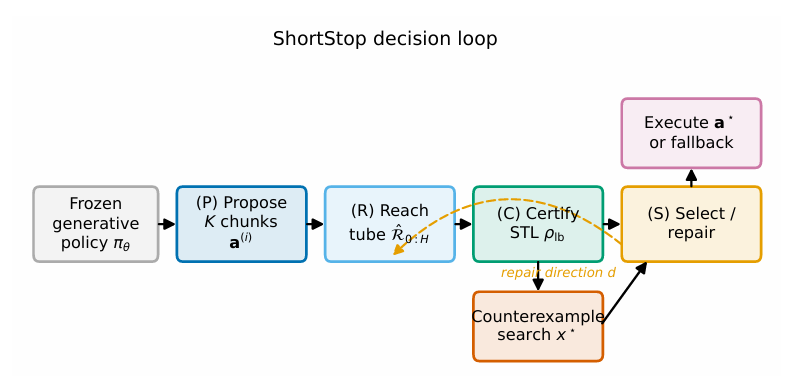
\includegraphics[width=0.5\linewidth]{images/shorstop_loop.png}
\end{center}

\vspace{2pt}
\footnotesize

\begin{itemize}
    \item \textbf{Predict}
    $\rightarrow$
    \textbf{Reachability analysis}
    --- set propagation (CORA, Flow*), cho ra một reachtube
    $\{\hat R_k\}$.

    \item \textbf{Certify}
    $\rightarrow$
    \textbf{Signal Temporal Logic (STL)}
    --- robustness định lượng được tính trên cả reachable tube,
    thay vì chỉ trên một trajectory nominal.

    \item \textbf{Repair}
    $\rightarrow$
    \textbf{CEGIS/CEGAR}
    --- dùng counterexample cụ thể để vừa bác bỏ candidate không an toàn,
    vừa định hướng sửa.

\end{itemize}

\end{frame}

\begin{frame}[t,shrink=8]{Các khối kiến thức có sẵn → SHORTSTOP (2/2)}

\begin{center}
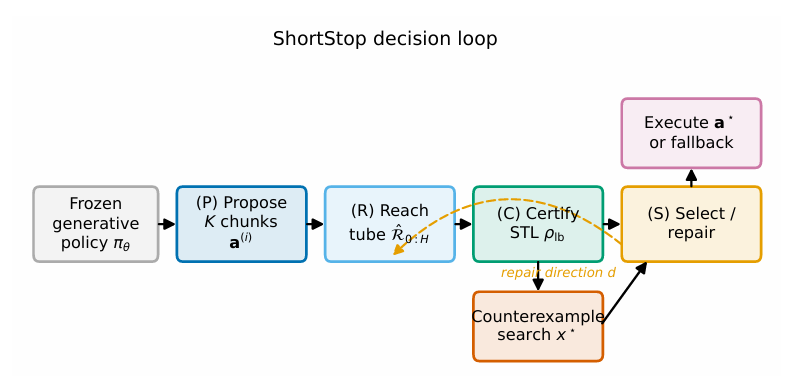
\includegraphics[width=0.5\linewidth]{images/shorstop_loop.png}
\end{center}

\vspace{3pt}

\begin{alertblock}{Đóng góp của SHORTSTOP}
Từng công cụ riêng lẻ đều là những khối kiến thức đã trưởng thành.
Đóng góp nằm ở việc \textbf{tích hợp chúng thành một runtime shield
counterexample-guided duy nhất} cho một generative policy đã đóng băng,
kèm safety guarantee cho từng quyết định.
\end{alertblock}

\end{frame}

%=====================================================================
\section{Part 4 --- The P-R-C-S Framework}
%=====================================================================

\begin{frame}[t,shrink=8]{SHORTSTOP: vòng lặp P-R-C-S}
\small
\begin{block}{Tại mỗi decision step $t$}
SHORTSTOP giữ nguyên policy $\pi_\theta$, lấy một batch candidate chunks, kiểm tra an toàn và chỉ cho phép chunk phù hợp được thực thi.
\end{block}
\vspace{-0.2em}
\begin{description}
    \item[\textbf{P} Propose:] Lấy $K$ candidate từ policy: $\{a^{(i)}\}_{i=1}^{K}\sim\pi_\theta(\cdot\mid o_t)$.
    \item[\textbf{R} Reach:] Lan truyền over-approximation trong short horizon:
    \[
        \hat{\mathcal R}_{k+1}=\hat f(\hat{\mathcal R}_k,a_{t+k})\oplus\mathcal B(\epsilon_k+\bar w).
    \]
    \item[\textbf{C} Certify:] Tính STL robustness-to-go lower bound trên tube: $\underline{\rho}=\rho(\varphi,\hat{\mathcal R})$.
    \item[\textbf{S} Select/Repair:] Nếu chưa đạt margin, tìm counterexample, sửa trong trust region rồi chọn chunk có task progress tốt nhất.
\end{description}
\end{frame}

\begin{frame}[t,shrink=8]{P-R-C-S: từ candidate chunk đến action thực thi}
\footnotesize
\setlength{\abovedisplayskip}{2pt}
\setlength{\belowdisplayskip}{2pt}
\setlength{\abovedisplayshortskip}{1pt}
\setlength{\belowdisplayshortskip}{1pt}
\begin{block}{Một decision step tại thời điểm $t$}
Policy sinh một \textbf{batch nhỏ} candidate chunks; SHORTSTOP chỉ filter các đề xuất này thay vì tìm toàn bộ action space.
\end{block}
\vspace{-0.5em}
\begin{columns}[T,onlytextwidth]

%---------------- LEFT ----------------
\column{0.48\textwidth}

\textbf{1. Propose}

$\{a^{(i)}\}_{i=1}^{K}\sim\pi_\theta(\cdot\mid o_t),\;K=8$

\textbf{2. Reach + Certify}

Mỗi candidate được:

\begin{enumerate}
    \setlength{\itemsep}{0pt}
    \item[(R)] propagate thành reachable tube;
    \item[(C)] tính STL robustness lower bound.
\end{enumerate}

$\underline{\rho}\geq\varepsilon\Rightarrow\textbf{certified admissible}$

%---------------- RIGHT ----------------
\column{0.52\textwidth}

\textbf{3. Select / Repair}

Nếu candidate không đạt chứng nhận:

$\underline{\rho}<\varepsilon$

SHORTSTOP:

\begin{enumerate}
    \setlength{\itemsep}{0pt}
    \item tìm một \textbf{counterexample}
    trong reachable tube;
    \item dùng nó để xác định hướng repair;
    \item sửa candidate trong trust region và quay lại \textbf{Reach}.
\end{enumerate}
Nếu có candidate admissible: $a^*=\arg\max_{a^{(i)}\in\mathcal C} g(a^{(i)})$, \textbf{chỉ action đầu tiên được execute}.\\
Nếu tất cả candidate đều fail: chuyển sang \textbf{safe fallback controller}, sau đó quan sát lại và re-plan.

\end{columns}
\end{frame}

%=====================================================================
\section{Part 5 --- Experimental Setup}
%=====================================================================

\begin{frame}[t,shrink=8]{Thiết lập thực nghiệm}

\begin{center}

\Large
\[
\boxed{
\text{Ở đâu?}
\quad
\boxed{\text{Stress thế nào?}}
\quad
\boxed{\text{So với ai?}}
\quad
\boxed{\text{Đo bằng gì?}}
}
\]

\end{center}

\vspace{8pt}

\begin{itemize}
    \item \textbf{Environments}: từ benchmark manipulation đến controlled
    reach-avoid setting.

    \item \textbf{Stress tests}: cố tình đưa policy ra khỏi nominal
    distribution.

    \item \textbf{Baselines}: cùng frozen generative policy, chỉ thay đổi
    safety mechanism.

    \item \textbf{Metrics}: đánh giá đồng thời safety, task performance,
    intervention quality và runtime cost.
\end{itemize}

\end{frame}

\begin{frame}[t,shrink=8]{Môi trường đánh giá: từ controlled đến realistic}

\begin{center}

\begin{tabular}{c|c|c}
\textbf{Testbed} & \textbf{Stress test cái gì} & \textbf{Vai trò} \\ \hline

LIBERO~[56]
&
Manipulation dài hạn (long-horizon)
&
Benchmark
\\[5pt]

ManiSkill2~[57]
&
Độ chính xác khi va chạm nhiều (contact-rich)
&
Benchmark
\\[5pt]

RLBench~[58]
&
Đa dạng tác vụ manipulation
&
Benchmark
\\[5pt]

Reach-Avoid-2D
&
Phân tích an toàn có kiểm soát
&
Soundness / prototype
\end{tabular}

\end{center}

\vspace{7pt}

\begin{alertblock}{Thiết lập chung}
Cùng một generative policy đã train bằng imitation learning và đóng băng
được bảo vệ bởi mỗi safety method. Không baseline nào được train lại policy riêng.
\end{alertblock}

\end{frame}

\begin{frame}[t,shrink=8]{Các môi trường đánh giá}

\begin{columns}[T]

\column{0.25\textwidth}
\centering
\textbf{LIBERO}\\
\small
Goal / Object / Spatial / Long

\column{0.25\textwidth}
\centering
\textbf{ManiSkill2}\\
\small
PickCube / StackCube / PegInsertion

\column{0.25\textwidth}
\centering
\textbf{RLBench}\\
\small
Reach / Close-box / Put-in-drawer

\column{0.25\textwidth}
\centering
\textbf{Reach-Avoid-2D}\\
\small
Nghiên cứu soundness có kiểm soát

\end{columns}

\vspace{10pt}

\begin{center}
\Large
\[
\text{Độ thực tế của benchmark}
\qquad\longleftrightarrow\qquad
\text{Phân tích có kiểm soát}
\]
\end{center}

\end{frame}

\begin{frame}[t,shrink=8]{Stress test: cố tình rời khỏi nominal distribution}

\begin{columns}[T]

\column{0.33\textwidth}

\textbf{1. Object-placement}

\begin{itemize}
    \item Vật cản / mục tiêu bị dịch chuyển
    \item Tối đa $\pm 6$ cm
    \item Đặt vị trí đối nghịch trên nominal path
\end{itemize}

\vspace{3pt}

\[
\boxed{\text{Sai lệch hình học}}
\]

\column{0.33\textwidth}

\textbf{2. Timing}

\begin{itemize}
    \item Jitter độ trễ điều khiển
    \item Rớt quan sát
    \item Lệch thời gian
\end{itemize}

\vspace{3pt}

\[
\boxed{\text{Sai lệch thời gian}}
\]

\column{0.33\textwidth}

\textbf{3. Visual-shift}

\begin{itemize}
    \item Thay đổi ánh sáng
    \item Thay đổi texture
    \item Nhiễu camera
\end{itemize}

\vspace{3pt}

\[
\boxed{\text{Sai lệch tri giác}}
\]

\end{columns}

\vspace{8pt}

\begin{alertblock}{Mục đích}
Stress test được thiết kế để tăng violation rate khi không có shield
(unshielded), và kiểm tra xem shield có can thiệp \textbf{chính xác}
hay chỉ đơn giản reject tất cả.
\end{alertblock}

\end{frame}

\begin{frame}[t,shrink=8]{Baselines: sáu hệ thống dưới cùng điều kiện}

\begin{center}

\begin{tabular}{c|l}
\textbf{Hệ thống} & \textbf{Cơ chế an toàn} \\ \hline

\texttt{Unshielded}
& Generative policy nguyên bản, không có shield
\\[3pt]

\texttt{Conf-Thresh}
& Reject chunk có độ bất đồng (disagreement) cao
\\[3pt]

\texttt{MPC-Filter}~[33]
& Sửa dự đoán có ràng buộc (constrained predictive correction)
\\[3pt]

\texttt{CBF-Shield}~[38,39]
& Barrier QP thiết kế tay
\\[3pt]

\texttt{STL-Monitor}~[53]
& Giám sát STL trên trajectory nominal
\\[3pt]

\textbf{SHORTSTOP}
& Reach + STL + repair theo counterexample
\end{tabular}

\end{center}

\vspace{7pt}

\begin{alertblock}{So sánh có kiểm soát}
Tất cả baseline dựa trên model đều dùng chung
$\hat f$, error bound $\epsilon$, policy checkpoint đã đóng băng,
và fallback controller.
\end{alertblock}

\end{frame}

\begin{frame}[t,shrink=8]{Metrics I --- Safety và chất lượng can thiệp}

\begin{columns}[T]

\column{0.5\textwidth}

\textbf{Safety}

\begin{itemize}
    \item \textbf{Violation rate}

    \[
    \%\,\text{episode đi vào }X_u
    \]

    Càng thấp càng tốt.

    \item \textbf{Task success}

    \[
    \%\,\text{episode hoàn thành nhiệm vụ}
    \]

    Càng cao càng tốt.
\end{itemize}

\column{0.5\textwidth}

\textbf{Chất lượng can thiệp}

\begin{itemize}
    \item \textbf{Shield activation rate}

    \[
    \%\,\text{quyết định bị reject/repair/fallback}
    \]

    Thường thì càng thấp càng tốt.

    \item \textbf{Intervention precision}

    Tỉ lệ can thiệp tương ứng với một vi phạm thật sự
    sẽ xảy ra.

    Càng cao càng tốt.
\end{itemize}

\end{columns}

\vspace{7pt}

\begin{alertblock}{Đánh đổi cốt lõi}
Một shield tốt cần giảm violation \textbf{mà không đơn giản là reject
tất cả}.
\end{alertblock}

\end{frame}

\begin{frame}[t,shrink=8]{Metrics II --- Chi phí runtime và giá trị can thiệp}

\begin{columns}[T]

\column{0.33\textwidth}

\textbf{Latency}

\[
\text{ms tăng thêm (trung vị) / quyết định}
\]

Đo overhead runtime.

\column{0.33\textwidth}

\textbf{Conservatism cost}

\[
\Delta\text{Success}
\]

trên các episode không có sự kiện an toàn thật sự.

Đo mức suy giảm hiệu năng không cần thiết.

\column{0.33\textwidth}

\textbf{Recovery rate}

\[
\frac{
\text{nhiệm vụ thành công sau can thiệp}
}{
\text{trường hợp chunk bị reject}
}
\]

Đo xem repair có phục hồi được hiệu năng nhiệm vụ hay không.

\end{columns}

\vspace{10pt}

\begin{alertblock}{Vì sao các metric này quan trọng}
Chỉ an toàn thôi là chưa đủ:
\[
\boxed{
\text{An toàn}
\;\not\Rightarrow\;
\text{Hữu ích}
}
\]

Một shield thực tế cần \textbf{an toàn, chọn lọc, phục hồi được, và nhanh}.
\end{alertblock}

\end{frame}

%=====================================================================
\section{Part 6 --- Guarantees \& Challenges}
%=====================================================================

\begin{frame}[t,shrink=8]{Vì sao khó để có được các guarantee này?}
\begin{itemize}
    \item \textbf{Epsilon calibration}: calibrate $\varepsilon$ đúng theo phân phối thật, không phải một hằng số cố định.
    \item \textbf{Model error dưới distribution shift}: $\varepsilon$ sai dưới shift $\Rightarrow$ certificate sập âm thầm mà không cảnh báo.
    \item \textbf{Safe fallback}: xây $X_s,\pi_{fb}$ hợp lệ --- không tự động đúng, phải thiết kế riêng.
    \item \textbf{Safety vs.\ liveness}: 22\% reject không recover; certify \emph{batch} chunk từ hộp đen.
    \item \textbf{Real-time constraint}: giải bài toán đối nghịch đủ nhanh \emph{và} đúng, trong ngân sách $<$10ms cạnh GPU policy.
\end{itemize}
\vspace{4pt}
\textit{3 lát cắt khó xuyên suốt: khái niệm (đúng ranh giới tractable/intractable), toán học (đúng đắn dưới bất định mà không biết cấu trúc $\pi_\theta$), hệ thống ($<$10ms cạnh GPU policy).}
\end{frame}

\begin{frame}[t,shrink=8]{Assumptions: điều kiện để guarantee đứng vững}
\begin{itemize}
    \item Mỗi challenge ở trên cần một giả định tương ứng để lý thuyết còn đứng vững:
    \item \textbf{Assumption 1}: reachable-set sound --- reachtube phải chứa quỹ đạo thật (đối phó với model error dưới distribution shift).
    \item \textbf{Assumption 2}: STL bound sound --- $\rho(\phi,\hat R)$ phải là cận dưới đúng của robustness thật (đối phó với sai số calibrate $\varepsilon$).
    \item \textbf{Assumption 3}: tồn tại safe fallback $(\pi_{fb}, X_s)$ --- luôn có đường lui an toàn (chính là challenge ``safe fallback'' ở trên).
    \item Mỗi assumption cũng bảo vệ đúng một mắt xích trong vòng P-R-C-S: (1)$\to$Reach, (2)$\to$Certify, (3)$\to$Select/Repair khi rỗng.
\end{itemize}
\end{frame}

\begin{frame}[t,shrink=8]{Từ Bounded-time đến All-time safety}
\begin{itemize}
    \item \textbf{Theorem 1} (bounded-time safety): với 3 assumption trên, chunk được ShortStop chấp nhận không vi phạm $X_u$ trong $H$ bước tới.
    \item \textbf{Corollary 1} (all-time safety): quy nạp theo $t$ dựa trên $X_s$ bất biến --- an toàn từng bước cộng dồn thành an toàn suốt quỹ đạo.
\end{itemize}
\end{frame}

\begin{frame}[t,shrink=8]{Conservatism vs. Horizon}
\begin{itemize}
    \item \textbf{Proposition 1} (Grönwall-type, Eq.~6--7): $r_k\le L^k r_0+(\varepsilon_{\max}+\bar w)\frac{L^k-1}{L-1}$, $\alpha(H)\le\alpha^\star+\beta(\epsilon+r_H)$.
    \item Đây chính là cơ sở toán học cho trực giác ``ngắn hạn vừa đủ vừa cần'' ở Part 3: $L^k$ tăng theo horizon $\Rightarrow$ tồn tại $H^\star$ tối ưu (thực nghiệm $H^\star=8$).
\end{itemize}
\end{frame}

%=====================================================================
\section{Track A \& Track B --- Kế hoạch song song}
%=====================================================================

\begin{frame}[t,shrink=8]{Track A \& Track B: hai kế hoạch chạy song song}
\begin{itemize}
    \item \textbf{Track A (Lý thuyết)}: Sec.~I--IV --- bài toán, related work, method, các định lý an toàn, chia theo 7 nhóm chủ đề.
    \item \textbf{Track B (Thực nghiệm)}: Sec.~V--VIII --- dựng pipeline trên \texttt{Reach-Avoid-2D} với policy Gaussian giả lập trước (stage 0--5), chỉ đưa generative policy thật vào từ stage 6a, rồi mới scale lên 3 benchmark thật (stage 7a--7c).
    \item \textbf{Vì sao chưa đụng generative policy ngay}: shield logic (reach/STL/CE-search/repair/baselines) cần debug nhiều vòng --- Gaussian rẻ và nhanh hơn; policy thật chỉ cần thiết khi kiểm tra đúng giả định ``black-box proposer''.
    \item 3 bảng dưới đây ghép mỗi stage Track B với nhóm lý thuyết Track A tương ứng, kèm status theo dõi.
\end{itemize}
\end{frame}

\begin{frame}[t,shrink=8]{Track A \& Track B: lộ trình song song (1/3)}
\footnotesize
\begin{tabularx}{\textwidth}{|>{\raggedright\arraybackslash}p{0.34\textwidth}|>{\centering\arraybackslash}p{0.09\textwidth}|>{\raggedright\arraybackslash}p{0.34\textwidth}|>{\centering\arraybackslash}p{0.09\textwidth}|}
\hline
\textbf{Track A} & \textbf{Status} & \textbf{Track B} & \textbf{Status} \\
\hline
\textbf{Stage 0} --- Reachability cơ bản (interval/zonotope, Minkowski sum, Lipschitz) + Shielding/Safe RL context (đọc nhanh). &
Đang thực hiện &
Setup --- env \texttt{Reach-Avoid-2D}, interval arithmetic, \texttt{cvxpy}; policy Gaussian giả lập chỉ để dựng khung. &
\good{Đã xong} \\
\hline
\textbf{Stage 1} --- Reachtube \& Assumption 1 (sound over-approximation). &
Chưa bắt đầu &
Reach-only shield --- reachtube, binary reject (Gaussian; violation $\approx3.8\%$, success $\approx64.1\%$). &
\good{Đã xong} \\
\hline
\textbf{Stage 2} --- STL syntax \& robustness-to-go, Assumption 2. &
Chưa bắt đầu &
STL-to-go --- thay reject nhị phân bằng robustness lower bound (Gaussian; kỳ vọng $\approx2.9\%$ violation). &
Chưa bắt đầu (tiếp theo) \\
\hline
\textbf{Stage 3} --- CEGIS: tìm counterexample (adversarial search). &
Chưa bắt đầu &
CE search --- projected gradient/vertex sampling trên box 2D (Gaussian; kỳ vọng $\approx1.7\%$ violation). &
Chưa bắt đầu \\
\hline
\end{tabularx}
\end{frame}

\begin{frame}[t,shrink=8]{Track A \& Track B: lộ trình song song (2/3)}
\footnotesize
\begin{tabularx}{\textwidth}{|>{\raggedright\arraybackslash}p{0.34\textwidth}|>{\centering\arraybackslash}p{0.09\textwidth}|>{\raggedright\arraybackslash}p{0.34\textwidth}|>{\centering\arraybackslash}p{0.09\textwidth}|}
\hline
\textbf{Track A} & \textbf{Status} & \textbf{Track B} & \textbf{Status} \\
\hline
\textbf{Stage 4} --- CEGIS: sửa theo counterexample (trust-region projection). &
Chưa bắt đầu &
Repair --- Algorithm~1 đầy đủ (Gaussian; kỳ vọng $\approx1.2\%$ violation). &
Chưa bắt đầu \\
\hline
\textbf{Stage 5} --- MPC/CBF \& fallback, Assumption 3 (safe fallback tồn tại). &
Chưa bắt đầu &
Baselines --- MPC-Filter, CBF-Shield, STL-Monitor, Conf-Thresh (vẫn trên Gaussian). &
Chưa bắt đầu \\
\hline
\textbf{Stage 6a} --- Generative policy, bản nhỏ (Diffusion Policy/flow matching). &
Chưa bắt đầu &
2D policy thật --- train một diffusion/flow policy nhỏ trên \texttt{Reach-Avoid-2D}, hoặc import policy có sẵn. &
Chưa bắt đầu \\
\hline
\textbf{Stage 6b} --- Safety guarantee (bounded-time $\to$ all-time, Grönwall trade-off). &
Chưa bắt đầu &
Metrics + stress test --- 7 metric, horizon sweep, bootstrap, \textbf{chạy lại với policy 2D thật thay Gaussian}. &
Chưa bắt đầu \\
\hline
\end{tabularx}
\end{frame}

\begin{frame}[t,shrink=8]{Track A \& Track B: lộ trình song song (3/3)}
\footnotesize
\begin{tabularx}{\textwidth}{|>{\raggedright\arraybackslash}p{0.34\textwidth}|>{\centering\arraybackslash}p{0.09\textwidth}|>{\raggedright\arraybackslash}p{0.34\textwidth}|>{\centering\arraybackslash}p{0.09\textwidth}|}
\hline
\textbf{Track A} & \textbf{Status} & \textbf{Track B} & \textbf{Status} \\
\hline
\textbf{Stage 7a} --- Generative policy, scale lên (cùng nhóm với 6a). &
Chưa bắt đầu &
\textbf{LIBERO} --- swap sang env thật, long-horizon manipulation. &
Chưa bắt đầu (tuỳ resource GPU) \\
\hline
\textbf{Stage 7b} --- Generative policy, scale lên (cùng nhóm với 6a). &
Chưa bắt đầu &
\textbf{ManiSkill2} --- swap sang env thật, contact-rich precision. &
Chưa bắt đầu (tuỳ resource GPU) \\
\hline
\textbf{Stage 7c} --- Generative policy, scale lên (cùng nhóm với 6a). &
Chưa bắt đầu &
\textbf{RLBench} --- swap sang env thật, diverse manipulation tasks. &
Chưa bắt đầu (tuỳ resource GPU) \\
\hline
\end{tabularx}
\vspace{4pt}
\footnotesize\textit{Số liệu LIBERO/ManiSkill2/RLBench trong Part 5 hiện là projection, không phải full simulator run --- stage 7a--7c chính là phần lấp khoảng trống đó.}
\end{frame}

%=====================================================================
\section{Tổng kết}
%=====================================================================

\begin{frame}[t,shrink=8]{Tóm tắt}
\begin{itemize}
    \item \textbf{Insight}: verify hậu quả ngắn hạn của 1 chunk, không verify cả policy.
    \item \textbf{Cơ chế}: reachtube sound + STL robustness-to-go + counterexample-guided reject/repair.
    \item \textbf{Bảo đảm}: bounded-time $\to$ all-time (recurrent fallback) $\to$ conservatism--horizon trade-off.
    \item \textbf{Kết quả (của paper)}: violation $18.7\%\to1.2\%$, giữ $92\%$ success, $+8.9$ms, precision $0.94$.
    \item \textbf{Vị trí}: điểm giao mới giữa 3 dòng nghiên cứu (post-hoc filter, reachability+STL, CEGIS) --- chưa ai làm cả ba cùng lúc cho generative robot policy.
    \item \textbf{Hướng tái lập và nghiên cứu tiếp theo}: Track A (lý thuyết, Module 1--4) + Track B (thực nghiệm, Phase 0--6) chạy song song --- Phase 0--1 đã xong, Phase 2 là bước tiếp theo.
\end{itemize}
\end{frame}

\end{document}
